% !TEX root = ../main.tex
\section{What Should We Do? Food Safety as Inspiration!}
\label{sec:inspiration}

As an inspiration for the technical, data-centric vision outlined in this paper, we discuss how the US Food \& Drug Administration (FDA) combats the outbreaks of foodborne illnesses~\cite{fdaout}, and start with a concrete example.

\subsection{Example -- Outbreak of Salmonella Infections in the US in 2020} 

From June to September in 2020, a total of 1,127 people in 48 US states got infected with the outbreak strain of Salmonella Newport~\cite{fdanewport}. The FDA and the Centers for Disease Control and Prevention (CDC) managed to contain this outbreak and had the situation under control in October 2020, after which no more new infections occurred. Combatting the outbreak proceeded as follows: Sick patients from the 48 states were seeking treatment in hospitals and bacteria in their stool samples turned out to be closely related genetically, which implied a common source of infection. Subsequent epidemiologic evidence showed that over 90\% of them had eaten onions (or food made with onions) in the week before their illness. As a consequence, the FDA started a so-called ``traceback investigation'' which ultimately uncovered that red onions from the Thomson International Inc. company were the source of the Salmonella outbreak. This triggered a country-wide recall of raw onions and derived products like cheese dips, kebabs, and chicken salad sandwiches from a large number of grocery stores, which ultimately ended the outbreak.



\subsection{Disease Detectives, Traceback Investigations, and Food Supply Chains}

The remarkable success of the FDA in combatting and controlling the salmonella outbreak naturally leads to the question which processes and techniques they have applied to detect the outbreak, identify the suspect food and determine the producer of the food, and what the computer science community can learn from these battle-tested approaches.

\begin{figure}[h!]
    \centering
    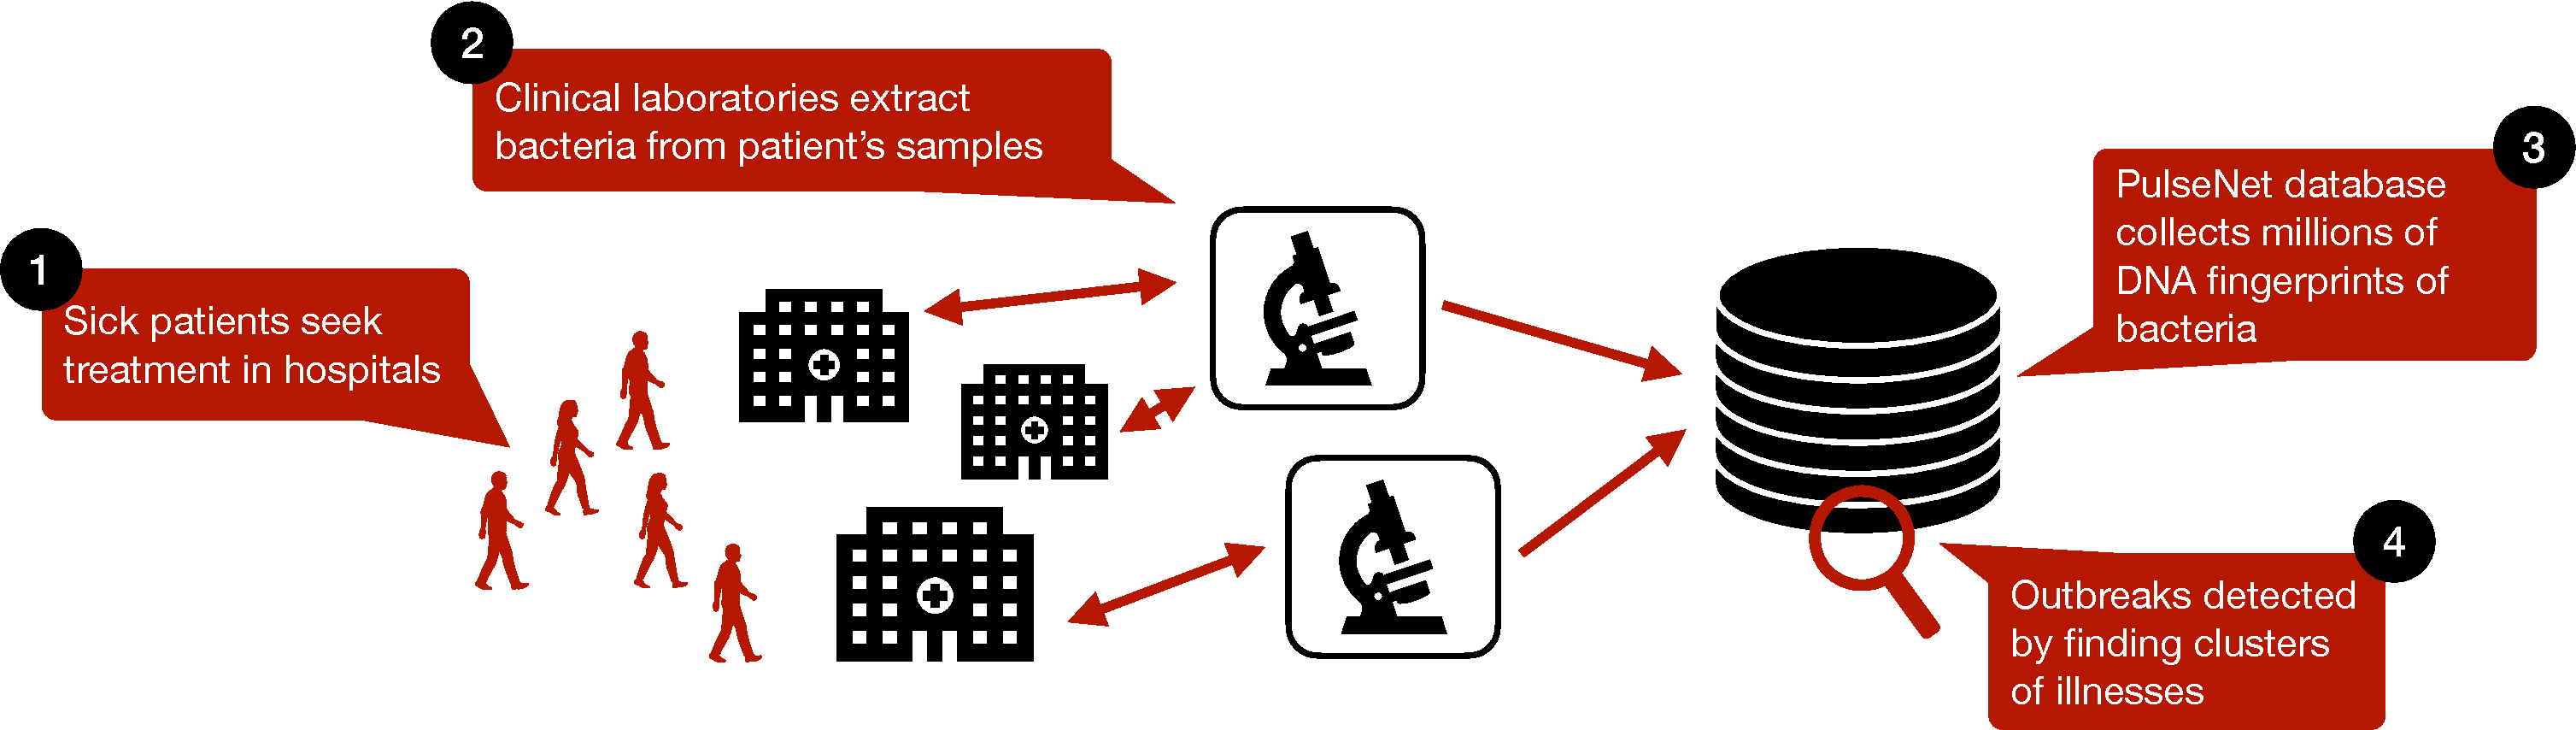
\includegraphics[width=0.8\textwidth]{submissions/submission3/figures/outbreak-detection-crop.pdf}
    \caption{Outbreak detection by monitoring a database of millions of DNA profiles of bacteria.}
    \label{fig:outbreak}
\end{figure}

\header{Outbreak detection} The first question is how the FDA actually detects that there is an outbreak of a foodborne disease. We illustrate the underlying process in \Cref{fig:outbreak}: Sick patients seek treatment in hospitals, from where their doctors send stool samples to laboratories for analysis. The laboratories perform DNA fingerprinting on the bacteria isolated from these samples via whole genome sequencing and the resulting DNA fingerprints are subsequently collected via the PulseNet system~\cite{cdcpulsenet}. PulseNet is a nationwide network of public health and food regulatory agency laboratories coordinated by the CDC and manages a national central database with millions of collected DNA profiles of bacteria. In this database, the sudden appearance of clusters of genetically related bacteria implies a common source of infection and indicates an outbreak.

\header{Identification of the suspect food} Once an outbreak is detected, the next task is to identify the contaminated ``suspect food'' which infects people. As shown in \Cref{fig:identification}, the FDA employs so-called ``disease detectives'', who contact the sick patients and interview them to gather epidemiologic evidence related to questions such as ``what foods did people eat before they got sick?'' or ``what restaurants, grocery stores, or events did sick people go to?''. For that, they leverage data provided by the patients, e.g., purchasing records collected on loyalty cards. These activities typically lead to the identification of a particular suspect food, which is likely the root cause of the outbreak.

\begin{figure}[h!]
    \centering
    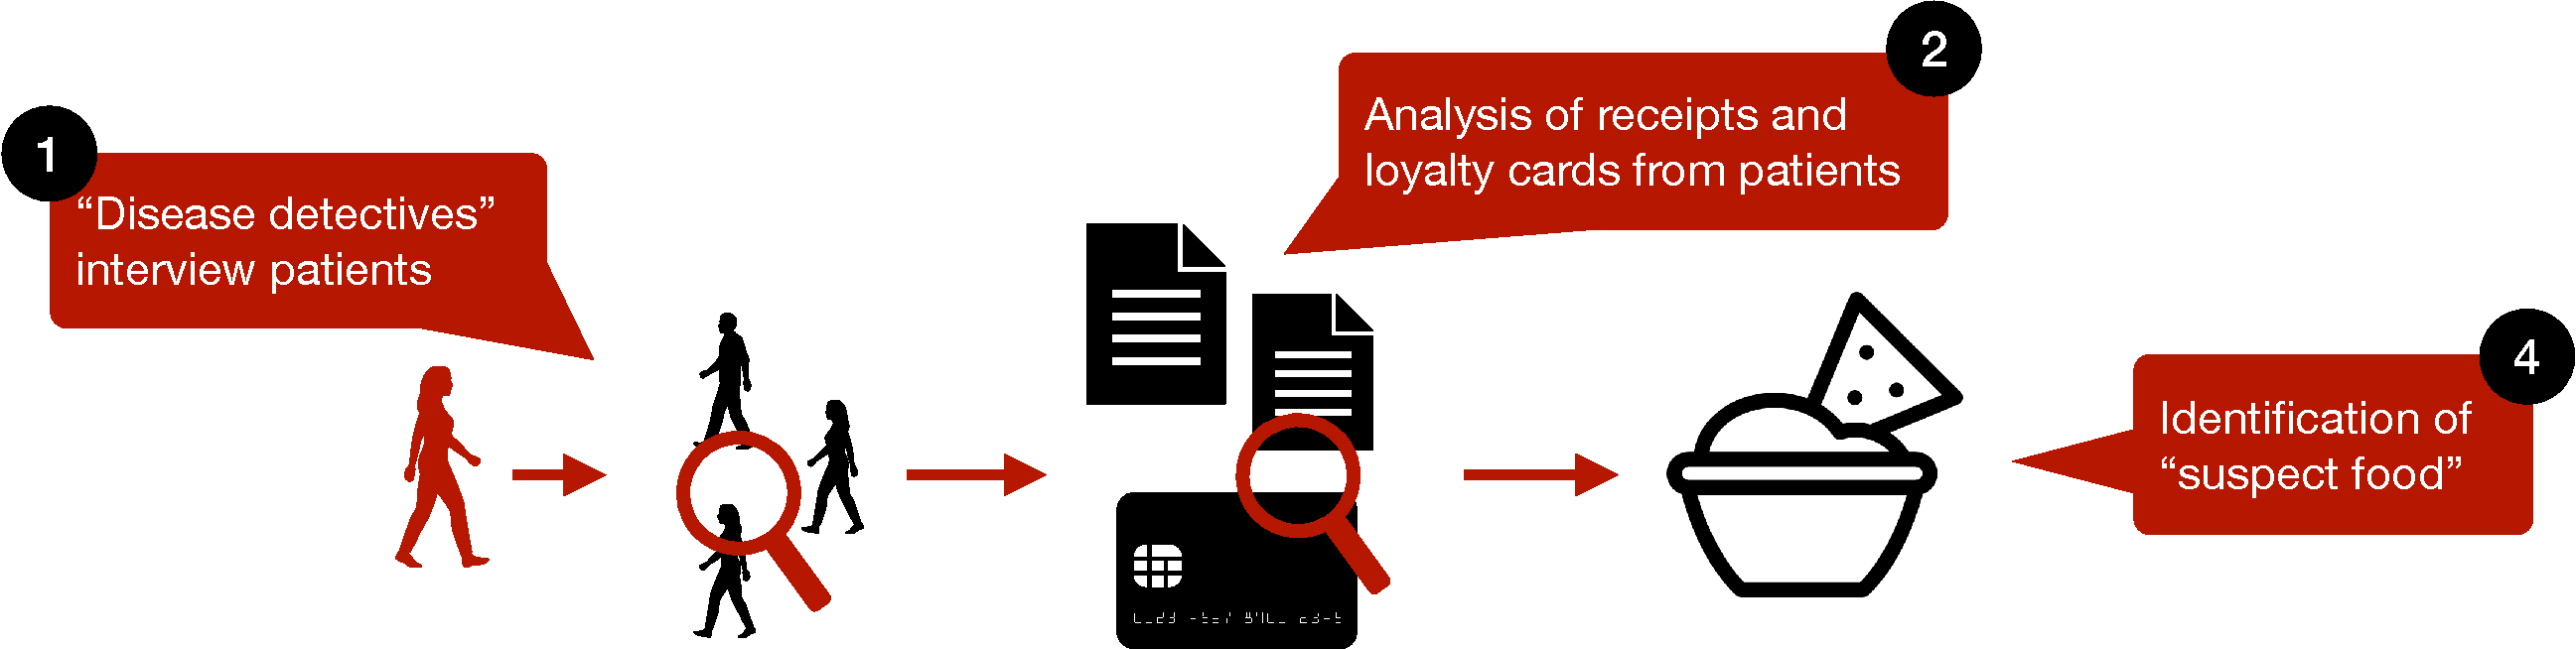
\includegraphics[width=0.8\textwidth]{submissions/submission3/figures/food-identification-crop.pdf}
    \caption{Disease detectives collect epidemiological evidence from sick patients to identify a contaminated suspect food likely causing the outbreak.}
    \label{fig:identification}
\end{figure}

\header{Traceback investigation to determine the producer of the contaminated food} Once the responsible food is known, the final task is to identify the actual point in the supply chain, where the food is likely being contaminated. For that, the FDA starts a traceback investigation through the food supply chain, as illustrated in \Cref{fig:traceback}. Here, the supply chain for several contaminated end products is traced back retrospectively to identify a common point in the supply chain which is likely the source of the contamination. 

\begin{figure}[h!]
    \centering
    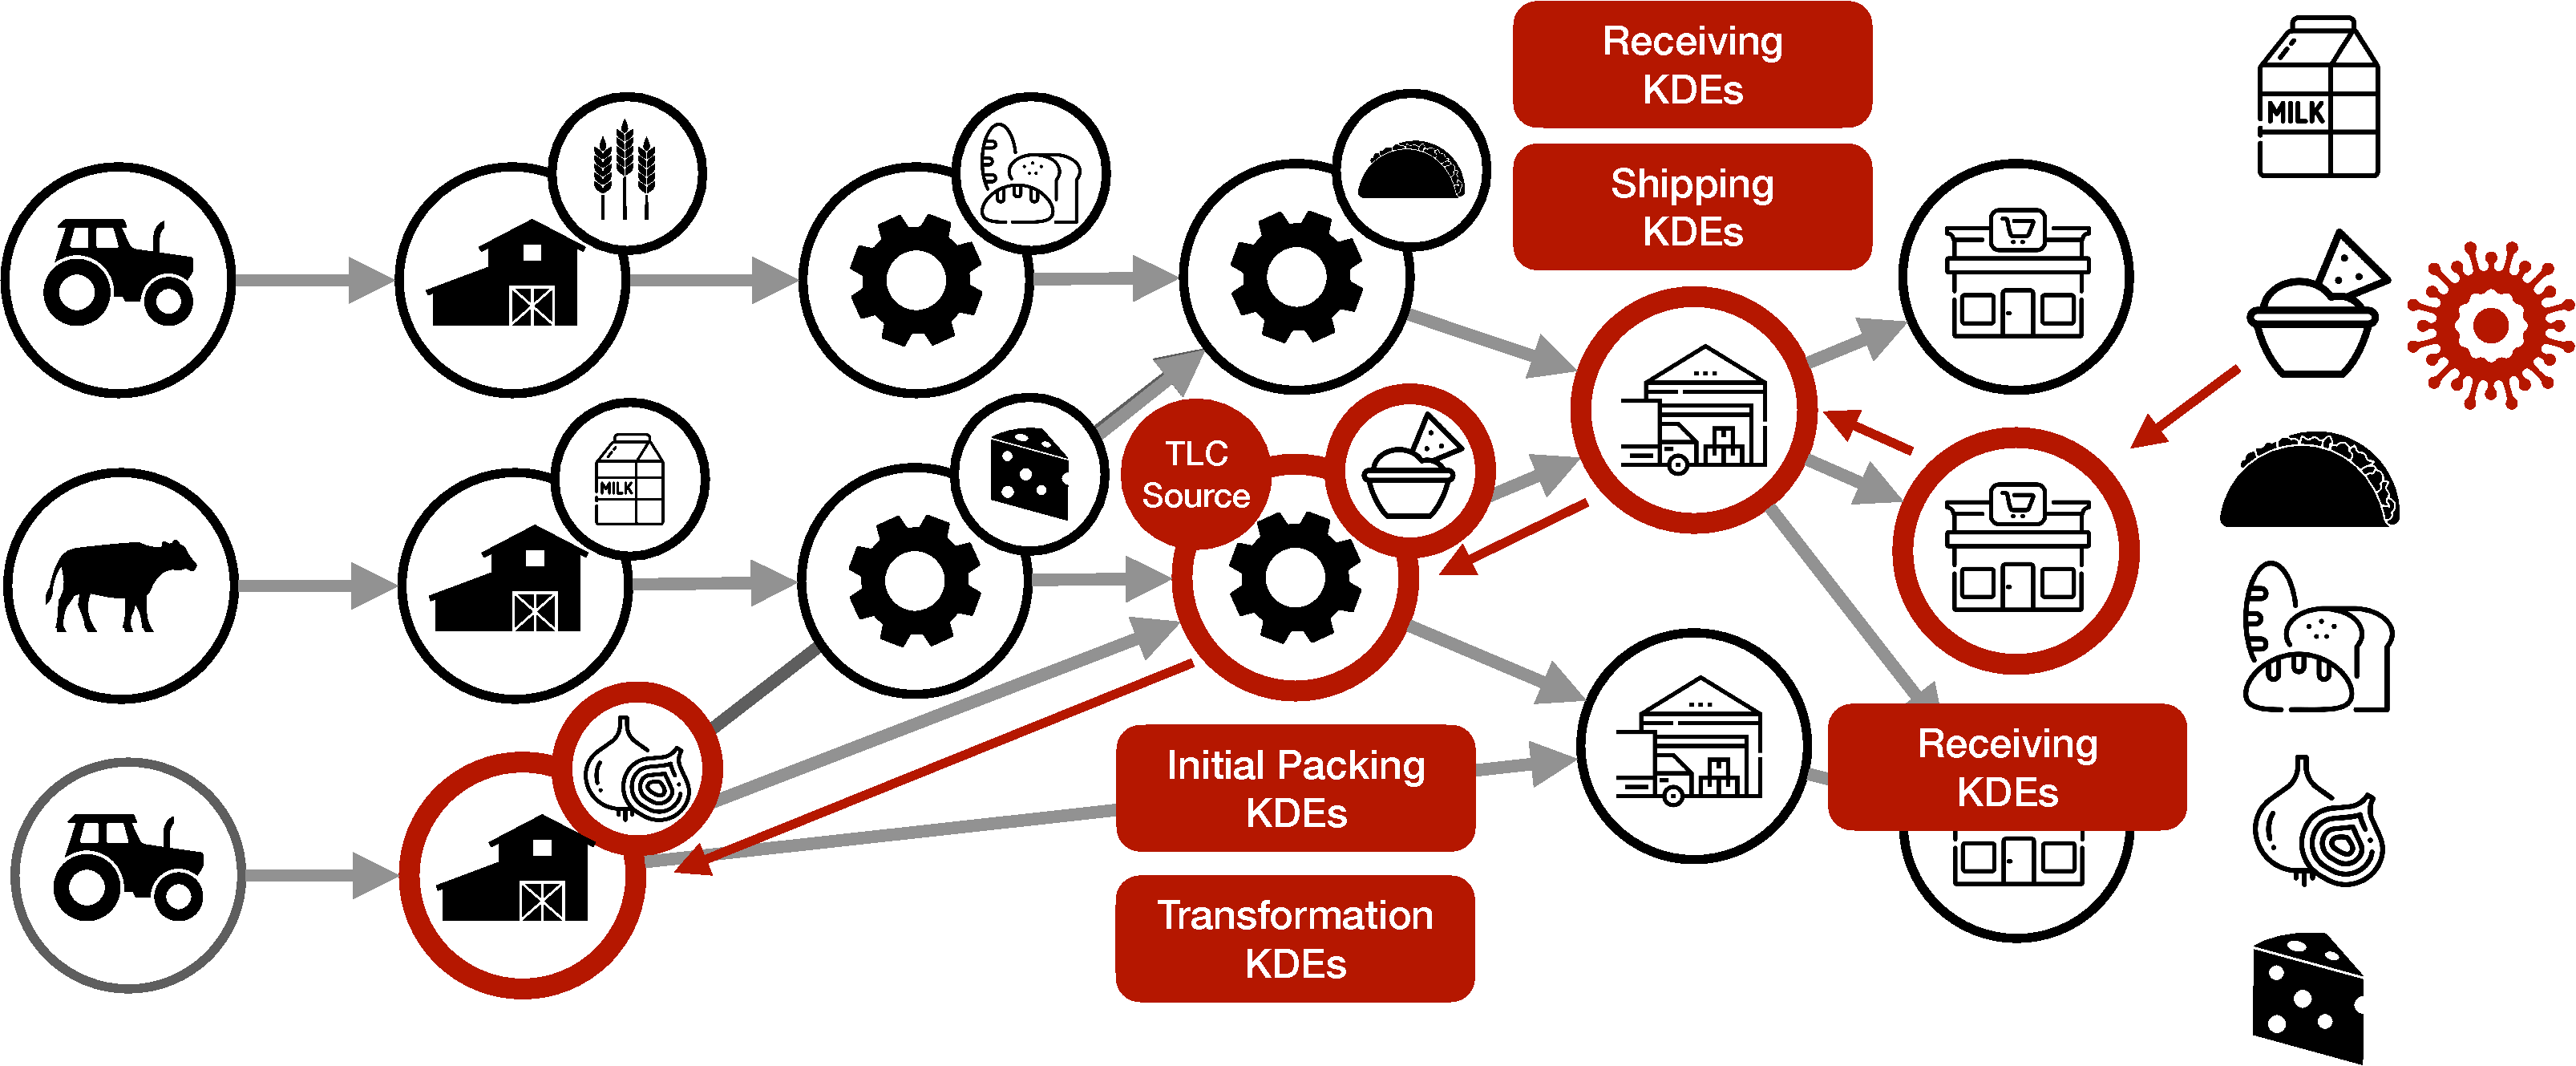
\includegraphics[width=0.8\textwidth]{submissions/submission3/figures/traceback-crop.pdf}
    \caption{Traceback investigation through the food supply chain, relying on \textit{Traceability Lot Codes} (TLCs) to identify units of food and provenance information in the form of \textit{Key Data Elements} (KDEs) to reconstruct the path a unit of food took through the chain.}
    \label{fig:traceback}
\end{figure}

For that to be possible, entities involved in the food supply chain must have followed the FDA's \textit{Food Traceability Rule}~\cite{fdafaq} and maintain traceability information for potentially dangerous food on the \textit{Food Traceability List}~\cite{fdaftl}. Such entities must maintain a \textit{Traceability Plan}, with information about procedures used to maintain traceability information and a point of contact for traceability questions~\cite{fdatp}. The food traceability rule further defines \textit{Critical Tracking Events} (CTEs) in the supply chain, where detailed tracing data must be created, maintained and forwarded by the participating entities. Examples of such events are the initial packing of a food, shipping it, or transforming multiple ingredients into a new food. An individual unit of food is assigned a \textit{Traceability Lot Code} (TLC),  typically during the initial packing event, which uniquely identifies it and is forwarded to receiving entities. Furthermore, the food traceability rule defines certain categories of \textit{Key Data Elements} (KDEs), which must be created, maintained, and forwarded together with the TLCs of the food. Examples of the different categories are \textit{Initial Packing KDEs}, \textit{Shipping KDEs}, \textit{Harvesting and Cooling KDEs} and \textit{Receiving KDEs}. The actual data items per KDE depend on the category, e.g., for the packing KDEs, the date, quantity, harvest location, name, and contact information of the harvesting company must be maintained, and the initial TLCs are typically assigned at the packing stage as well. Shipping KDEs need to include the corresponding TLCs, the shipping date, and the locations for receiving and shipping. A special case are Transformation KDEs, which must be created at points where a new food is produced from several ingredients. Here, the link to the ingredient TLCs must be recorded, as well as a location description, the transformation date, and the quantities of the ingredients.
